\ifgerman{\chapter{Evaluierung}}{\chapter{Evaluation}}
\label{evaluation}
We have performed various experiments in order to evaluate our Semantic Document Matching approach using Apache Spark. The details about the experimental procedure as well as the results obtained are discussed in this chapter. \ref{Section: Experimental Setup} provides information about the environmental setup used for the evaluation. In \ref{section: input dataset}, we discuss the details of the input dataset used for evaluations.

\section{Experimental Setup}
\label{Section: Experimental Setup}

In this section, We provide the details about the spark cluster as well as about the various size of the input data that are used for evaluations.

\subsection{Environment}

Evaluations are performed on a spark cluster that composes of 7 worker node and a master node. As mentioned earlier in \ref{section: management of clusters}, a spark program can be run either in a local mode or in a cluster mode. Cluster managers are required if a program needs to run in cluster mode and hence spark provides standalone cluster manager as well as supports other cluster managers includes Hadoop YARN and MESOS. We discuss about the software and hardware configurations of the cluster in the following sections.

\textbf{Hardware Configuration} 
\par As stated above, we have used a cluster consisting of 7 worker nodes and a master node. Each worker posses 4 processing cores and 6 Gigabytes of main memory. Though all the workers posses quad core processors but are in heterogeneous in nature. 

\textbf{Software Configuration}
\par We used Open VPN and SSH Secure shell to establish a connection to the cluster and also to upload the input dataset to the local file system. Every worker in the cluster has the following software installed on them:
\begin{itemize}
\item Ubuntu 64-bit operating system
\item PySpark 2.2.0
\item Python 2.7
\item Java 1.8
\end{itemize}


\subsection{Input Dataset}
\label{section: input dataset}
We have used Reuters corpus version1 (rcv1) to perform evaluations. The detailed discussions are pointed in \ref{section: rcv1}. Rcv1 totally contains 806791 documents organized into 365 folders. The total size of the corpus is 3.67 Gigabytes. To perform various evaluations, all the documents in the corpus are separated with varying sizes and are illustrated in \ref{tab:input dataset with various size}. 

\begin{table}[htbp]
	\centering
		\begin{tabular}{cc}\toprule
		Number of Documents in Input Dataset & Size in MB\\\midrule
		\(10^4\) & 29 \\\addlinespace 
		\(2*10^4\)  &  59 \\\addlinespace
        \(3*10^4\)  &  89 \\\addlinespace
        \(4*10^4\)  &  116 \\\addlinespace
        \(5*10^4\)  &  147 \\\addlinespace
        \(6*10^4\)  &  176 \\\addlinespace
        \(7*10^4\)  &  207 \\\addlinespace
        \(8*10^4\)  &  236 \\\addlinespace
        \(9*10^4\)  &  263 \\\addlinespace
        \(10^5\)  &  296 \\\bottomrule
		\end{tabular}
	\caption{A Table illustrating input dataset with various size}
	\label{tab:input dataset with various size}
\end{table}

\section{Experimental Procedure}
To evaluate the thesis and to optimize the implementation process, we have performed various experiments using the different sizes of the input dataset as shown in \ref{tab:input dataset with various size}. The cluster setup has also been varied according to the requirement of the experiment. In this section, We discuss the details of the experiments performed and how the procedure is carried out. 


\subsection{Experimental Procedure for Evaluation of Speed-up and Efficiency }
The primary focus of the thesis is to decrease the execution time of the Semantic Document Matching process in a parallel environment. To analyze the parallelism achieved by the implementation process, We have calculated the Speed-up and Efficiency. We have evaluated the approach with varying number of worker nodes ranging from 2 to 7 in the cluster and the memory usage of each worker node is set to 6 Gigabytes. To analyze the parallelism of the implementation process, we require a large voluminous input dataset. Hence we have evaluated this experiment with the input dataset consisting of \(10^5\) documents as shown in \ref{tab:input dataset with various size}.  

\par The evaluation is carried out by calculating the total execution time taken by the approach starting from the loading stage to the classification stage. We have not considered the evaluation stage for this experiment. The results obtained for the experiment are discussed in \ref{subsection: evaluating speed-up and efficiency}.

\subsection{Experimental Procedure for Evaluation of Threshold based Classification }

To analyze the parallelism achieved by the classification stage, we performed this experiment with varying amounts of input dataset using 7 worker nodes in the cluster. The varying amounts of input dataset are illustrated in \ref{tab:input dataset with various size}. The worker nodes are not varied in this experiment. With this experiment, the total runtime taken by the implementation process for classification stage is calculated and the results obtained are discussed in \ref{subsection: evaluating threshold}.


\subsection{Experimental Procedure for Effectiveness Evaluation}

The aim of this experiment is to evaluate the quality of the results obtained by the entire Semantic Document Matching process. As discussed earlier in \ref{section: rcv1}, the input dataset Reuters Corpus Version 1 (rcv1) do not possess any information on the ground truth describing the semantic similarity between two documents. Hence, we have designed a workaround method and the detailed discussion can be found in \ref{implement:evaluation}. The ground truth table was generated by implementing the workaround method for \(10^4\) documents and is used for this experiment. The quality measures like precision, recall, and F-measure are calculated. The obtained results are discussed in \ref{subsection: evaluating effectiveness}.


\section{Evaluation Results and Discussion}

In this section, we discuss the results obtained for the above discussed experiments.

\subsection{Evaluating Speed-up and Efficiency}
\label{subsection: evaluating speed-up and efficiency}

By varying the worker nodes of the cluster, We have evaluated the runtime, speedup, and efficiency of the Semantic Document Matching process. The runtime of the approach was calculated from starting of spark context till the classification stage. On one worker node, it took 55 minutes to process the \(10^5\) documents. It is then reduced to 18 minutes on an average when run on 4 worker nodes but again increased. When the application was run on 7 workers nodes of the cluster, the execution time was reduced to 14 minutes on an average. The execution time for varying number of worker nodes is illustrated in \ref{fig: result_runtime}. But on performing optimizations on the implementation process, we have succeeded in further reducing the execution time of the process and is illustrated in \ref{fig: result_improved_runtime}. The performed optimizations are discussed in \ref{section: Discussions}.

\begin{figure}[htbp]
	\centering
		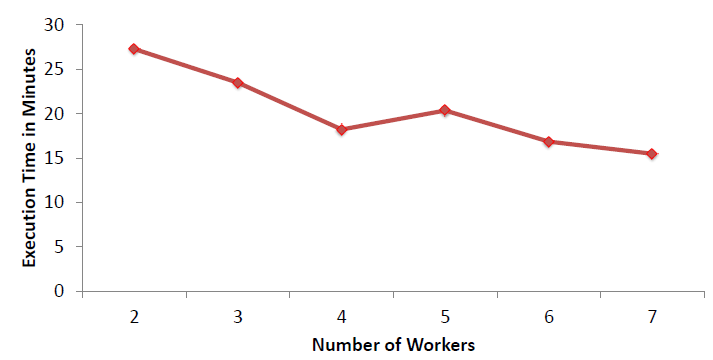
\includegraphics[scale=0.80]{runtime_result}
	\caption{Execution Time for processing \(10^5\) documents, Topics (K) = 90, Iterations = 20, Vocabulary Size = 137462, Total Document Pairs Classified =  4999950000}
	\label{fig: result_runtime}
\end{figure}

\begin{figure}[htbp]
	\centering
		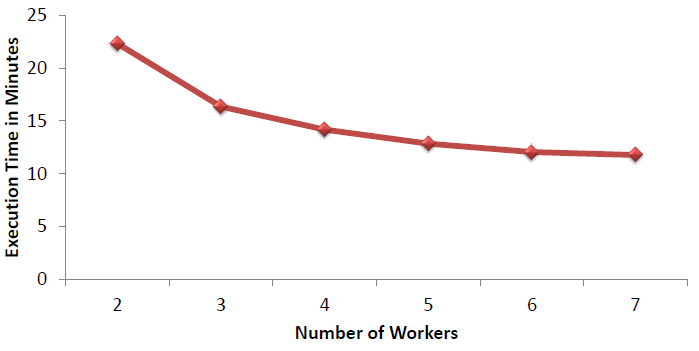
\includegraphics[scale=0.80]{improved_runtime}
	\caption{Improved Execution Time for processing \(10^5\) documents, Topics (K) = 90, Iterations = 20, Vocabulary Size = 137462, Total Document Pairs Classified =  4999950000}
	\label{fig: result_improved_runtime}
\end{figure}


\begin{figure}[htbp]
	\centering
		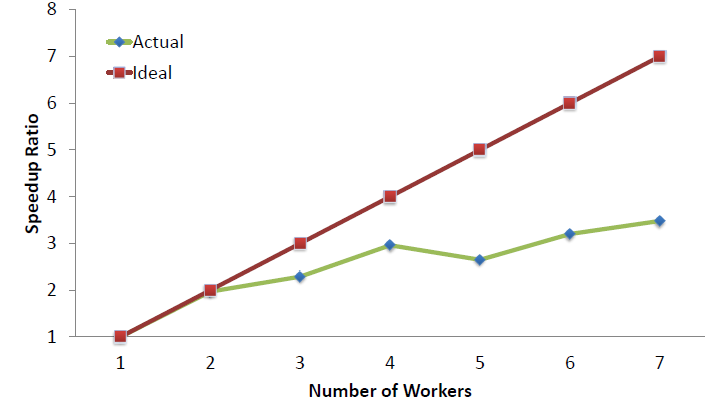
\includegraphics[scale=0.80]{speedup}
	\caption{Speedup for dataset size \(10^5\), Topics (K) = 90, Iterations = 20, Vocabulary Size = 137462, Total Document Pairs Classified =  4999950000}
	\label{fig: result_speedup}
\end{figure}

\begin{figure}[htbp]
	\centering
		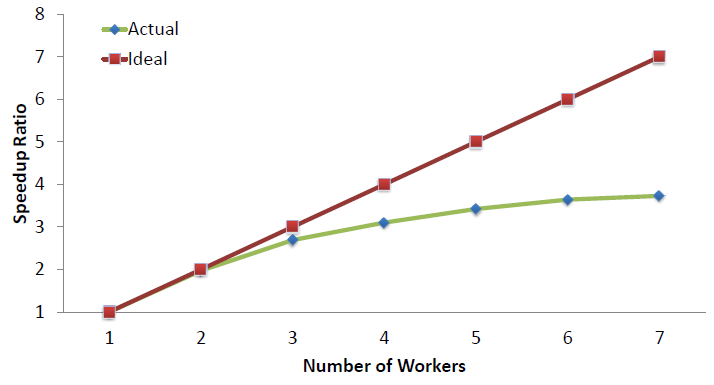
\includegraphics[scale=0.80]{improved_speedup}
	\caption{Improved Speedup for dataset size \(10^5\), Topics (K) = 90, Iterations = 20, Vocabulary Size = 137462, Total Document Pairs Classified =  4999950000}
	\label{fig: result_improved_speedup}
\end{figure}

\begin{figure}[htbp]
	\centering
		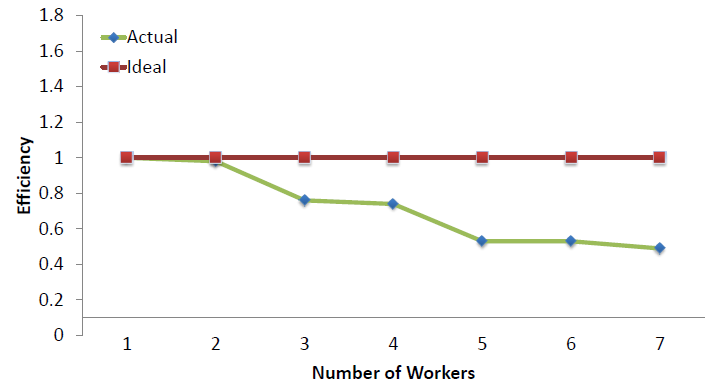
\includegraphics[scale=0.80]{Efficiency}
	\caption{Efficiency for dataset size \(10^5\), Topics (K) = 90, Iterations = 20, Vocabulary Size = 137462, Total Document Pairs Classified =  4999950000}
	\label{fig: result_efficiency}
\end{figure}

\begin{figure}[htbp]
	\centering
		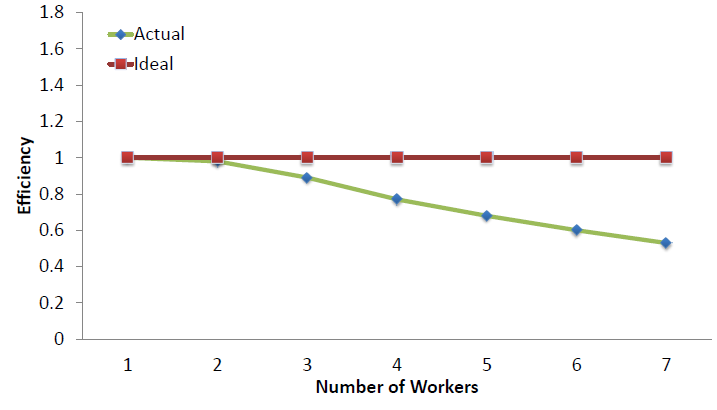
\includegraphics[scale=0.80]{improved_Efficiency}
	\caption{Improved Efficiency for dataset size \(10^5\), Topics (K) = 90, Iterations = 20, Vocabulary Size = 137462, Total Document Pairs Classified =  4999950000}
	\label{fig: result_improved_efficiency}
\end{figure}


\par Based on the execution time of the Semantic Document Matching process, the speedup and efficiency of the approach are calculated as per the evaluation metrics discussed in \ref{section: evaluation}. The results obtained on calculating efficiency and speed up can be observed in \ref{fig: result_speedup} and \ref{fig: result_efficiency}. We only ran 20 iterations on the input dataset as our primary focus is to increase the efficiency of the implementation but not calculating the convergence. As the execution time of the implementation has improved after performing optimizations, we have the improved speedup and efficiency for the same dataset and parameters respectively. The improved speedup and efficiency can be observed in \ref{fig: result_improved_speedup} and \ref{fig: result_improved_efficiency} respectively.

\subsection{Evaluating Threshold based Classification}
\label{subsection: evaluating threshold}

From \ref{fig: result_runtime_classification}, we can observe the total runtime taken by the document matching process for different datasets using a cluster with 7 worker nodes. To process \(10^4\) documents, on an average it took 7 minutes for the cluster to classify the documents and the execution time is increased for processing \(10^5\) documents to 13 minutes. The execution time taken to process \(10^5\) documents got faster when compared to the execution time taken to process \(10^4\) documents. This is due to only a few executors were assigned for the tasks by the YARN cluster manager for processing smaller datasets where as every worker was assigned a job in processing \(10^5\) documents. From \ref{tab:document pairs classified by threshold based classification}, we can observe the total number of document pairs classified based on the threshold value in the classification stage.

\begin{figure}[htbp]
	\centering
		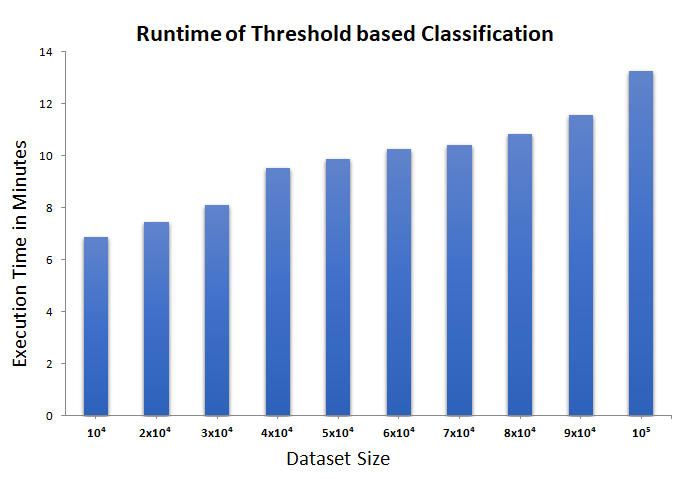
\includegraphics[scale=0.80]{runtime_threshold_classification}
	\caption{Runtime of Threshold based Classification for varying datasets}
	\label{fig: result_runtime_classification}
\end{figure}

\begin{table}[htbp]
	\centering
		\begin{tabular}{cc}\toprule
		Number of Documents in Input Dataset & Total Document Pairs Classified\\\midrule
		\(10^4\) & 49995000 \\\addlinespace 
		\(2*10^4\)  &  199990000 \\\addlinespace
        \(3*10^4\)  &  449985000 \\\addlinespace
        \(4*10^4\)  &  799980000 \\\addlinespace
        \(5*10^4\)  &  1249975000 \\\addlinespace
        \(6*10^4\)  &  1799970000 \\\addlinespace
        \(7*10^4\)  &  2449965000 \\\addlinespace
        \(8*10^4\)  &  3199960000\\\addlinespace
        \(9*10^4\)  &  4049955000 \\\addlinespace
        \(10^5\)  &  4999950000 \\\bottomrule
		\end{tabular}
	\caption{A Table illustrating document pairs classified by threshold based classification}
	\label{tab:document pairs classified by threshold based classification}
\end{table}


\subsection{Evaluating Effectiveness}
\label{subsection: evaluating effectiveness}

The aim of this evaluation is to verify and compare the quality of the results obtained from the Semantic Document Matching process with the generated golden data. On comparing the results obtained from classification stage to the golden data, We have evaluated this experiment by classifying the obtained results as true positives, true negatives, false positives, and false negatives in the evaluation stage. Based on these classifications, the quality measures like precision, recall, and f-measure are calculated for the input dataset consisting of \(10^4\) documents. The results of precision, recall, and f-measure are illustrated in \ref{tab:fmeasure}. 

\begin{table}[htbp]
	\centering
		\begin{tabular}{cccc}\toprule
		Number of Documents in Input Dataset & Precision & Recall & F-measure\\\midrule
		
        \(10^4\)  &  0.366 & 0.168 & 0.230 \\\bottomrule
		\end{tabular}
	\caption{A Table illustrating Effectiveness measures}
	\label{tab:fmeasure}
\end{table}

\subsection{Discussions}
\label{section: Discussions}

\textbf{Speedup and Efficiency}

\par From \ref{fig: result_runtime}, we can observe that the execution time is reduced rapidly as the number of worker nodes increased but then suddenly increased. On analyzing we found that the increase of execution time occurred because the input data is not distributed equally to all the worker nodes in the cluster. Hence we have performed the following optimizations to achieve better efficiency

\begin{itemize}
\item The default Java serialization is changed to kryo serializer which helps in faster serialization as per the official apache spark suggestion \cite{spark:website}.
\item With the help of repartition() method, the data is distributed equally among all the worker nodes in the cluster by specifying the number of partitions. The method is invoked every time when the data is loaded into a DataFrame using Spark SQL. The number of partitions is specified in proportion to the number of cores that are set while executing the implementation process.
\end{itemize}

\par Usually it takes \(O(n^2)\) computations to perform document pair comparison. However by defining a join condition as discussed in \ref{implement: Document Pair Comparison}, we have achieved the good results in reducing the number of computations required in comparing the document pairs and is illustrated in \ref{fig: result_runtime_classification}.

\par Though we have achieved some improvement in increasing the efficiency of the Semantic Document Matching process on applying the above optimizations, but are not appreciable when compared to the ideal efficiency and speedup and the same can be observed from \ref{fig: result_improved_efficiency} and \ref{fig: result_improved_speedup}. In general, the ideal efficiency achieved should be constant with the increase of worker nodes in the cluster. But the efficiency we have obtained for our approach is dropped with the increase of worker nodes in the cluster. We analyze that the reason for the loss of efficiency is due to heterogeneous nature of the cluster. At the driver node, most of the time is lost in waiting for some of the executors in the completion of tasks as the heavy computations need to be performed for generating the similarity score for two documents.




\textbf{Effectiveness}

From \ref{tab:fmeasure}, we can observe that the accuracy obtained by the Semantic Document Matching process is very poor. We analyze the following are major reasons for poor accuracy:

\begin{itemize}
\item The focus of the thesis is primarily on increasing the efficiency of the implemented process. As a result, the perplexity of the LDA modeling techniques and model fitting was not measured because the efficiency degrades with the increase in accuracy of the output data.

\item As discussed in earlier sections, the input dataset rcv1 do not provide any information on ground truth representing the similarity between two documents. Therefore, we have designed a workaround method and is discussed in \ref{implement:evaluation} to generate golden data. But we observed that the implemented workaround method is still not perfect as some of the labels generated in golden data contain null values as some of the documents in rcv1 do not possess the topic information. The presence of null values decreases the accuracy.
\end{itemize}

\par The workaround method was not improved further due to the limitation of thesis period. The semantic similarity obtained by the Document Matching process speaks about how two documents are semantically similar but the golden data represents only about the overlap of topics between two documents. Hence, the results obtained cannot be compared to golden data. But we have presented the results to address the existing problems in calculating the accuracy.

%Die Beurteilung ist einer der wichtigsten Abschnitte der Arbeit
%- Sie enthält die Quintessenz des gesamten Projektes
%Viele lesen nur die Einführung und die Beurteilung an
%- Hier muss also alles Wichtige drin stehen!
%Hier beweisen Sie dass Sie …
%- die Aufgabe und deren Bedeutung verstanden haben
%- die Ergebnisse richtig zu interpretieren vermögen
%- wissen, worauf es bei diese Arbeit ankam

